% !TEX root = report.tex

\section{Processing Pipeline}
\label{sec:processing_architecture}

High level descripion of the processing flow:

Throughout the report: extract Spectrograms, classify image.

\section{Signals and Features}
\label{sec:model}

\subsection{Google Dataset}

% Measurement setup, data preprocess (describe the google dataset)

The Speech Commands datasets, described in \cite{warden2018speech}, provides
thousands of one second recording of $35$ differen words. The recordings are
mainly of volounteers, who used their own device to record the words in a
closed room wherever they happened to be (not in a studio setting).
Ideally each volounteer only recorded the $135$ requested utterances once, so the
dataset provides good variability of voices.
The utterances have a duration of one second.
To more precisely align the recorded clips, the audio was acquired for $1.5$
seconds and the $1$ second clip that contained the highest overrall volume was
extracted.
Several background noise recording are included as well.
The full dataset includes $105829$ utterances of $35$ words, saved in
\textit{.wav} format at $16$ KHz rate.
The dataset is released under the Creative Commons BY $4.0$ License \cite{ccby4}.

The dataset ships with a function to split the data in train, validation and
test folds, as well as two example lists of validation data ($9981$ utterances)
and test data ($11005$ utterances).
Throughout the experiments, those lists were used.
% MAYBE both for the practicality of having them ready, but also to keep with
% the spirit of the dataset as a tool to enable meaningf

% TODO: how the words are grouped, tell the keys

Smaller tasks were used to evaluate the performance of the various
architectures, and to perform the hyper-parameter search.
Two 4 words task are composed by the words
[\texttt{happy}, \texttt{learn}, \texttt{wow}, \texttt{visual}],
[\texttt{backward}, \texttt{eight}, \texttt{go}, \texttt{yes}].
A 6 words task contains the direction words:
[\texttt{up}, \texttt{down}, \texttt{forward}, \texttt{backward},
\texttt{left}, \texttt{right}]
Two 10 words task contains the number utterances:
[\texttt{zero}, \texttt{one}, \texttt{two}, \texttt{three}, \texttt{four},
\texttt{five}, \texttt{six}, \texttt{seven}, \texttt{eight}, \texttt{nine}]
and the words from a Kaggle competition aimed at solving this task:
[\texttt{yes}, \texttt{no}, \texttt{up}, \texttt{down}, \texttt{left},
\texttt{right}, \texttt{on}, \texttt{off}, \texttt{stop}, \texttt{go}]
and a 20 words task is composed by the numbers and the Kaggle list.

\subsection{Mel spectrogram and Mel-frequency Cepstral Coefficients}

The audio data in the dataset is available as a vector of amplitudes over time,
sampled at $16$ KHz. In this representation, the classification task is quite
hard.
The Fourier transform allows to convert a signal from the time domain into the
frequency domain. The result is called spectrum of the signal. This transform
is efficiently computed using the Fast Fourier Transform algorithm.

The short-time Fourier transform accounts for variations of the content of an
audio signal over time. Instead of computing the FFT of the entire signal, the
FFT is computed on overlapping windowed segments of the signal: each window has
length \texttt{n\_fft} and the next window is extracted after
\texttt{hop\_length} samples.
The results of the FFT in each window are stacked to obtain the spectrogram.

The human ear does not perceive frequencies on a linear scale: the difference
between $200$ and $400$ Hz is very marked, whereas two notes at $8000$ and
$8200$ Hz are almost indistinguishable. The mel scale, proposed by Stevens,
Volkmann, and Newmann \cite{melscale1937}, introduces a unit of pitch built in
such a way that equal distances on the scale sound equally distant to the human
listener.
The mel spectrogram is a spectrogram where the frequencies are converted to the
mel scale. To do so, a Mel spaced filterbank is generated (a 10 filters version
is shown in \fig{fig:mel10_filterbank}) and the FFT results are multiplied with
a dot product with each filter, obtaining \texttt{n\_mel} values for each
timestep.

\begin{figure}[t!]
    \centering
    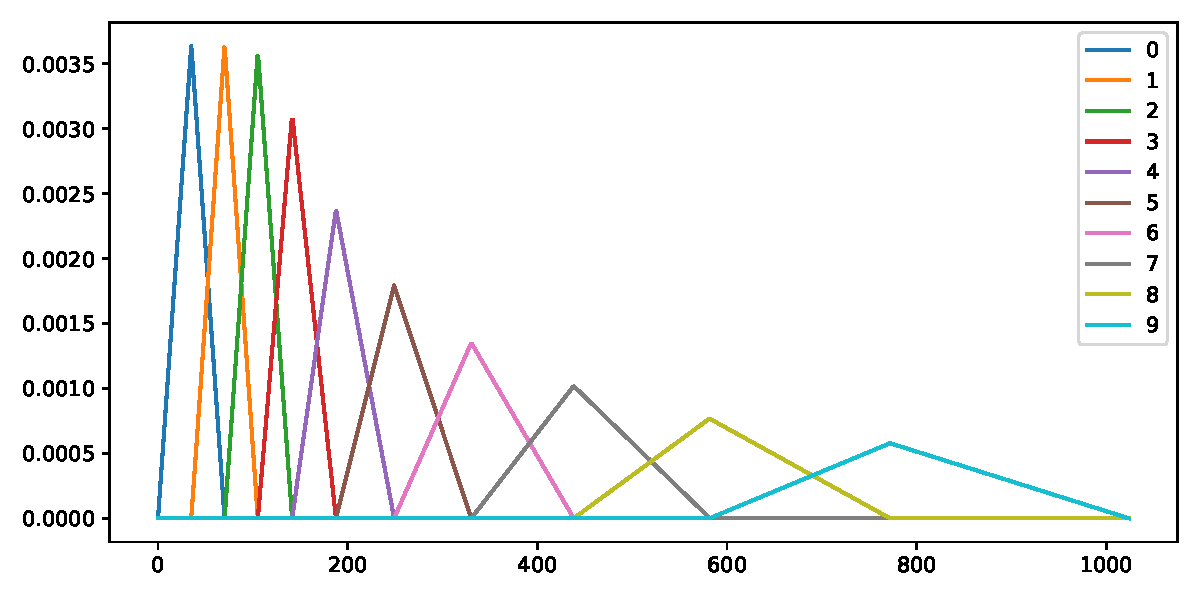
\includegraphics[width=0.9\linewidth]{mel10_filterbank.pdf}
    \caption{An example of a 10 filters Mel filterbank}
    \label{fig:mel10_filterbank}
\end{figure}

The resulting coefficients are highly correlated: the Discrete Cosine Transform
can be applied to decorrelate the filter bank coefficients and obtain a
compressed representation.
The results are the Mel-frequency Cepstral Coefficients.

The spectrograms were obtained using the \texttt{librosa} library
\cite{brian_mcfee_2020_3955228}.
The values used to generate the mel spectrograms are listed in
\tab{tab:mel_values}.
The values used to generate the mel frequency cepstral coefficients are listed
in \tab{tab:mfcc_values}.
An example waveform for the word ``happy'' and the relative spectrograms are
shown in \fig{fig:happy_specs}.

Some of the architectures that were tested require a square image as input,
with three color channels.
To obtain them, some spectrogams were purposefully generated with parameters
that created a square result, others, shaped like a half square, were
concatenated, as shown in the ``melc1'' spectrogram in
\fig{fig:happy_mel01_mel04_mel06_melc1_specs}.
Three square spectrogams are then stacked depthwise to obtain a valid three
channel image.
The values used to compose the spectrogams are listed in \tab{tab:compose_values}.
The values used to stack the spectrogams are listed in \tab{tab:ch3_values}.

\begin{figure}[t!]
    \centering
    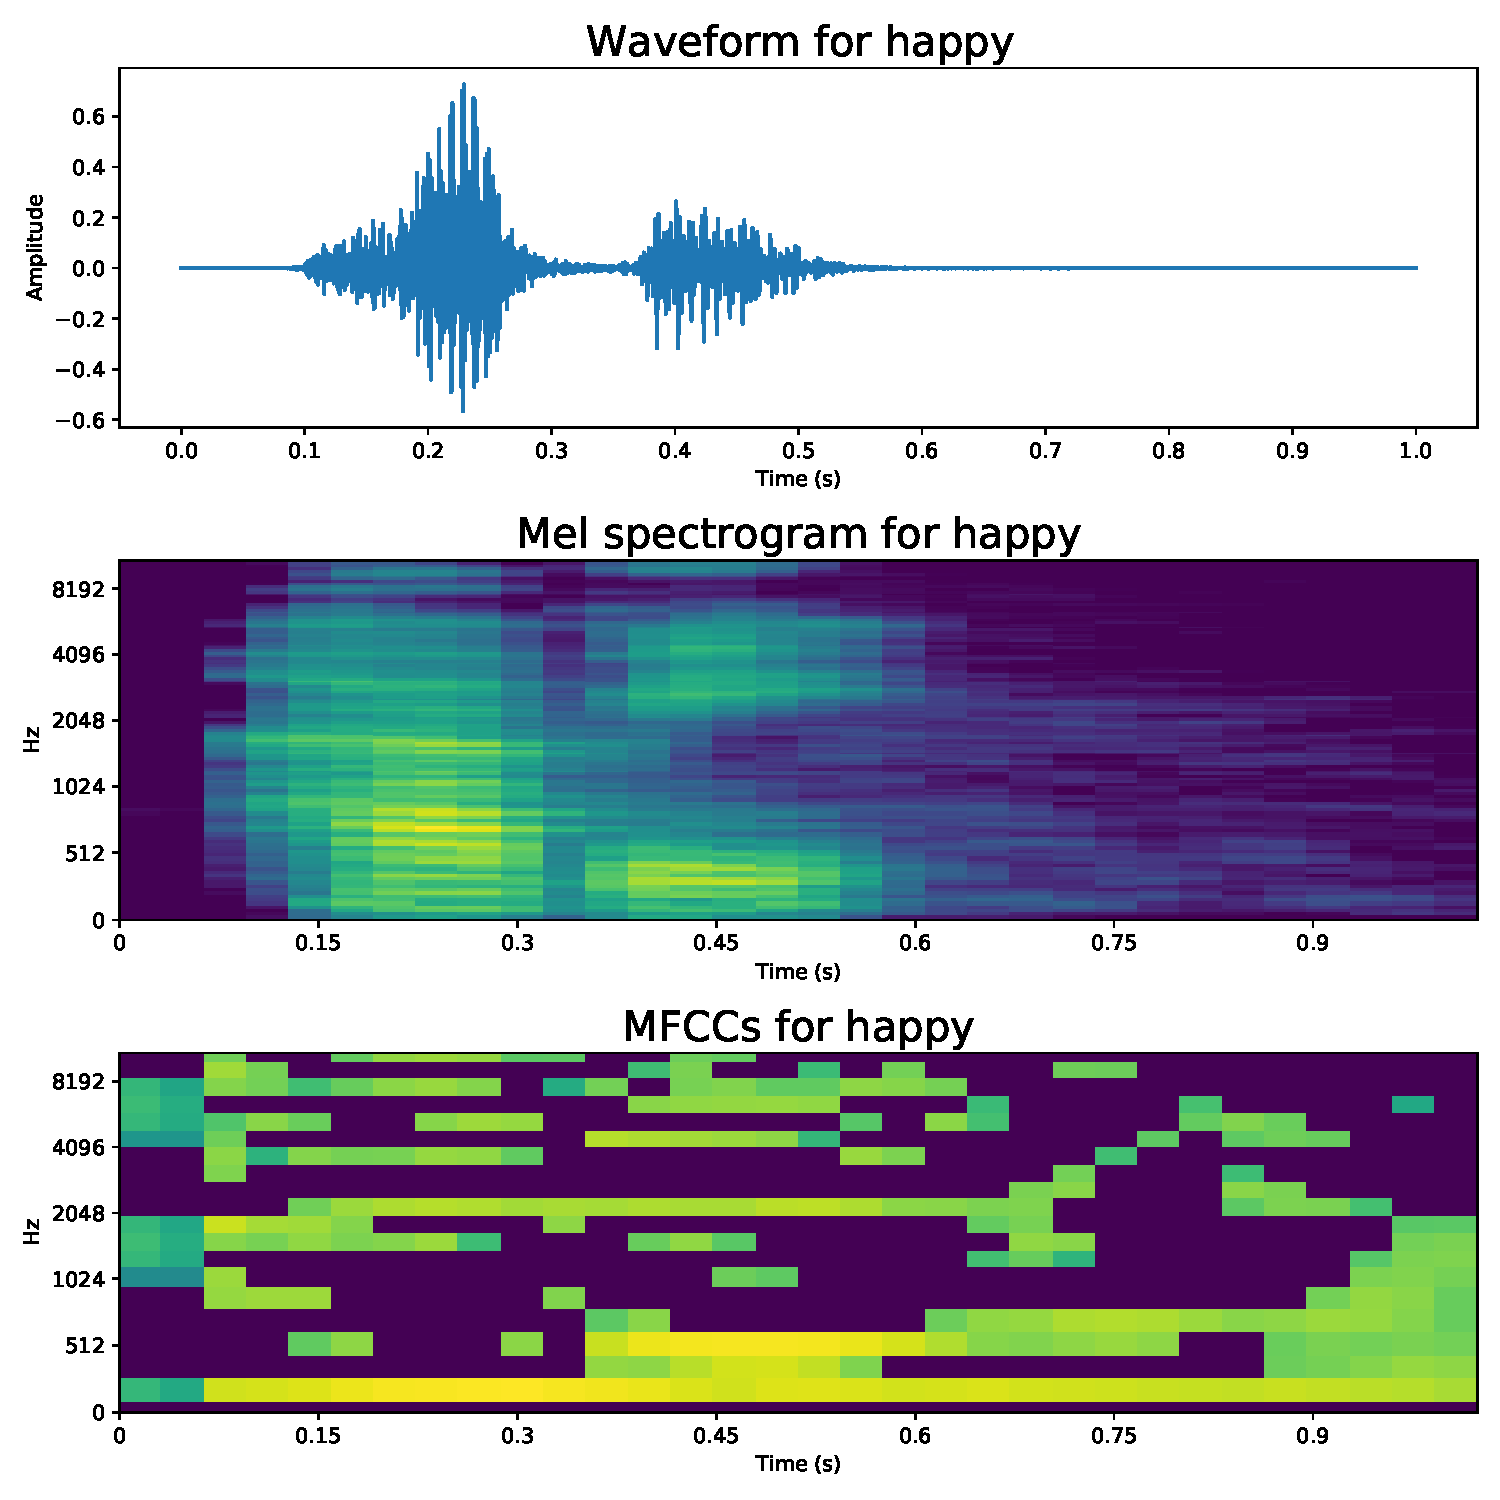
\includegraphics[width=0.9\linewidth]{happy_specs.pdf}
    \caption{
    Waveform and spectrograms for the word happy. Note that the y axis of the
spectrograms are labeled as Hz, but this is only to read more easily the plot
and understand to which frequencies the important bins correspond to. }%
    \label{fig:happy_specs}
\end{figure}

\begin{figure}[t!]
    \centering
    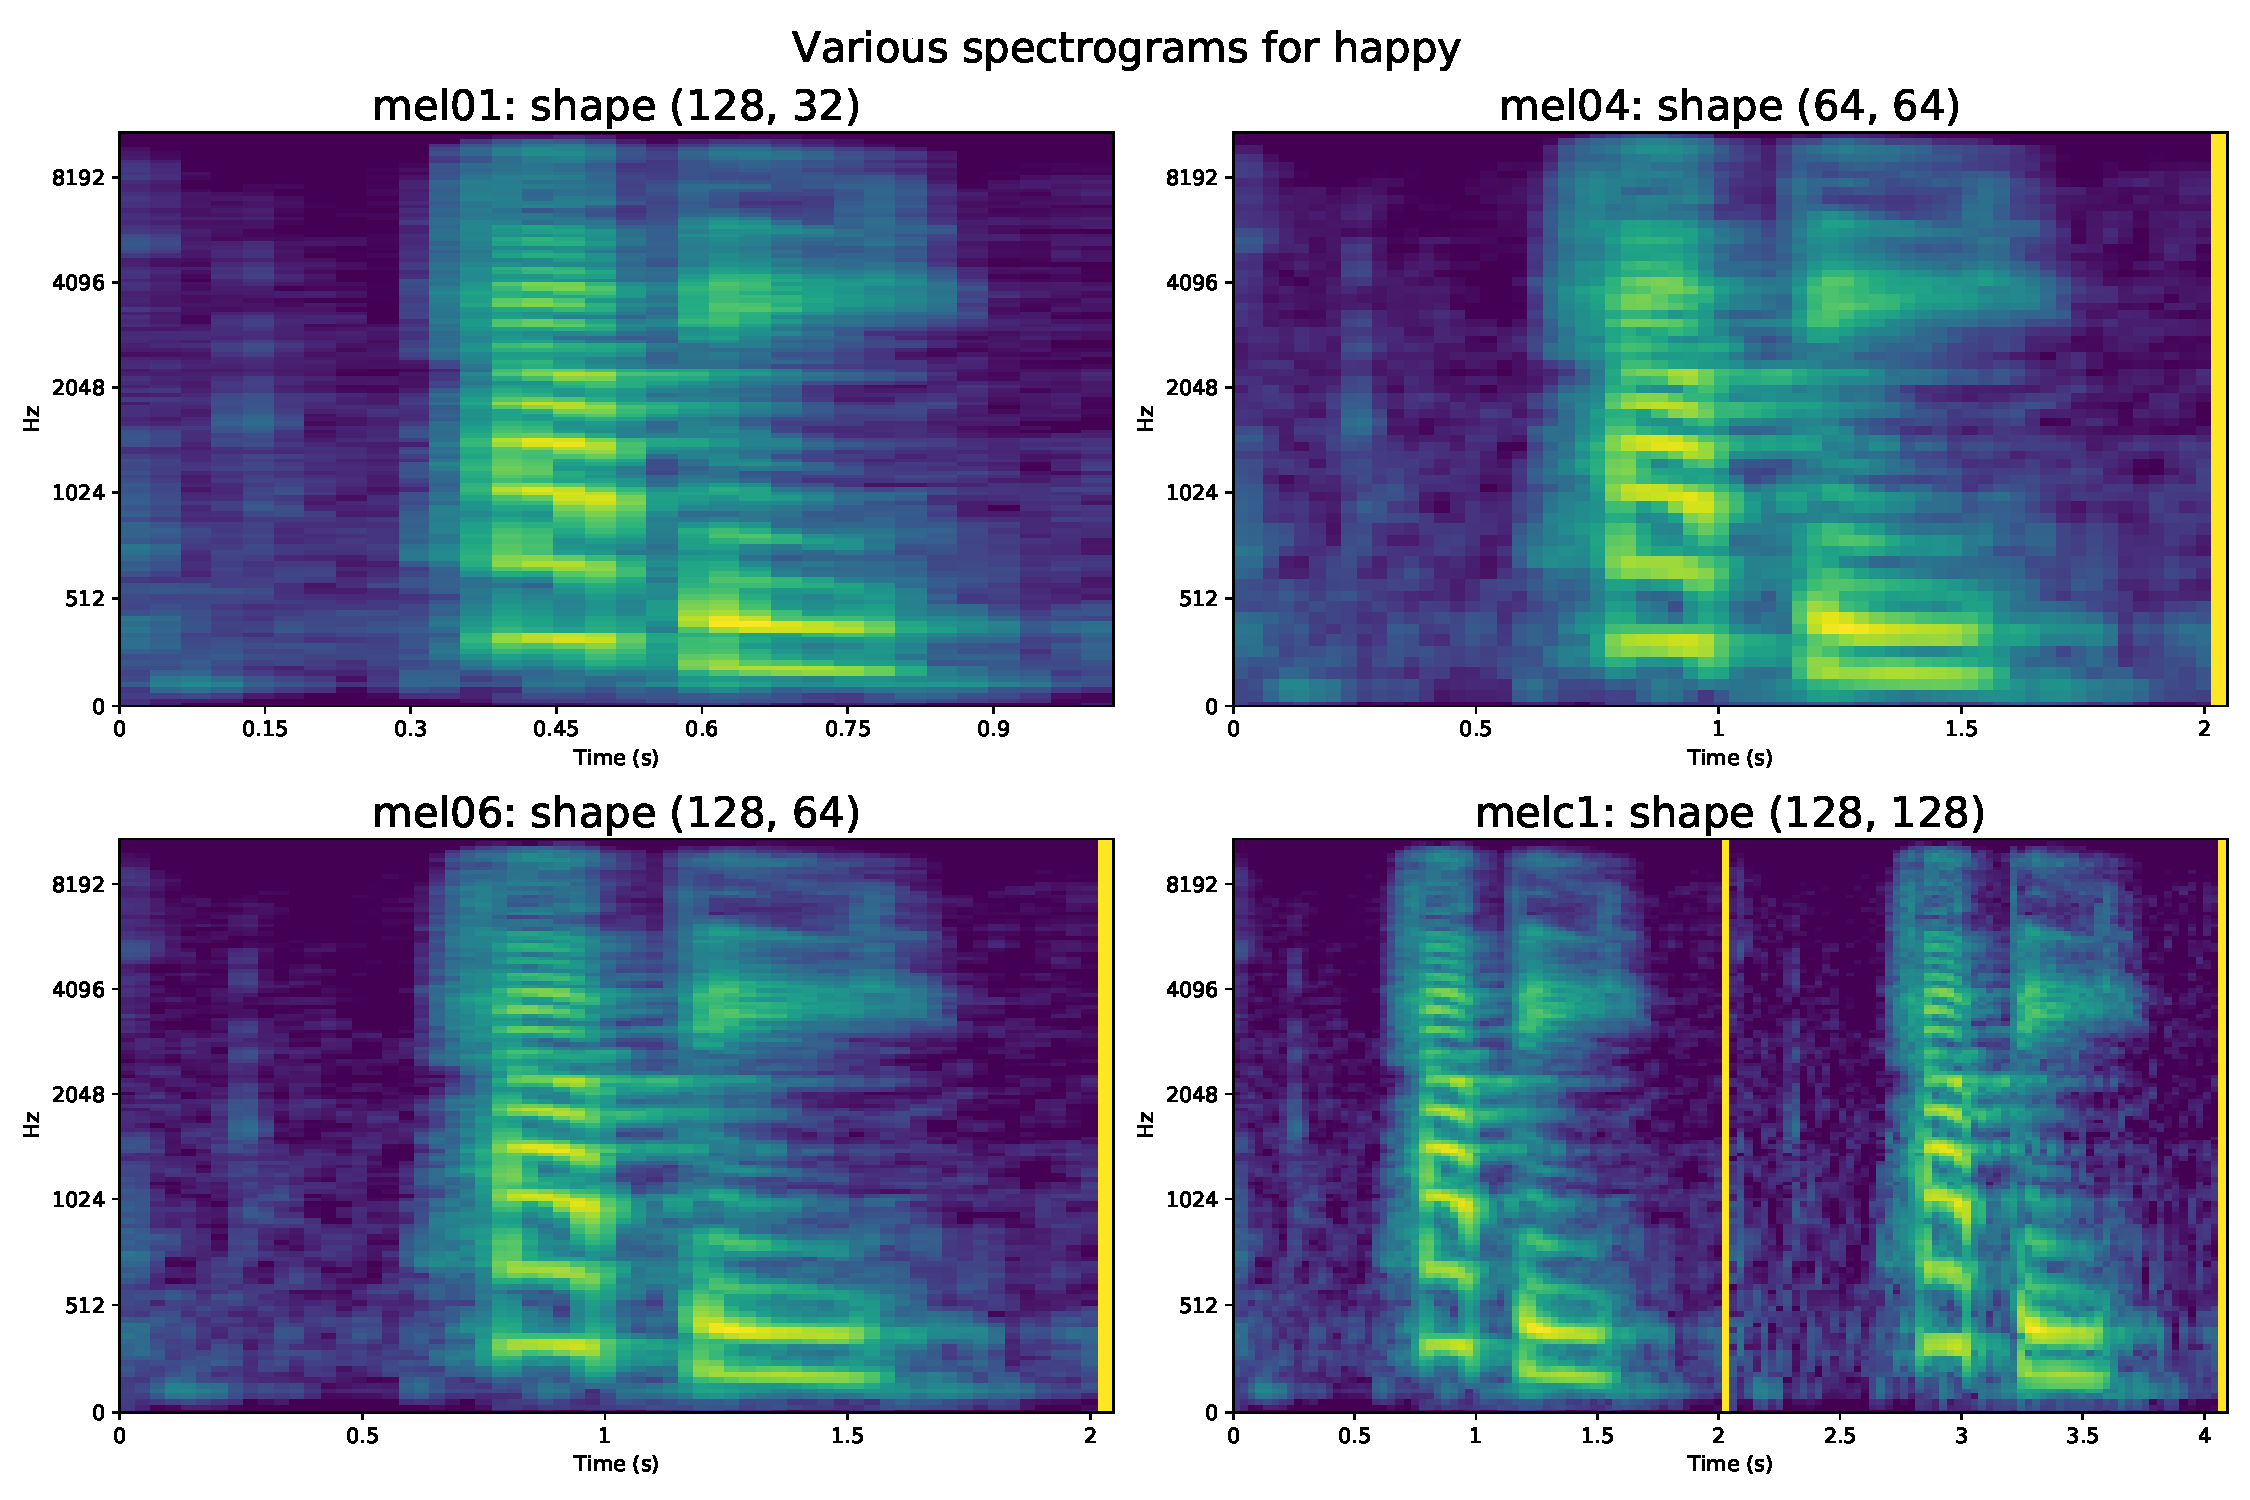
\includegraphics[width=0.9\linewidth]{happy_mel01_mel04_mel06_melc1_specs.pdf}
    \caption{Different spectrograms for the same word}%
    \label{fig:happy_mel01_mel04_mel06_melc1_specs}
\end{figure}

TODO: decision of preprocessing the data separately.

\subsection{Data augmentation}

Data augmentation is a technique to increase the amount of data available by
applying random, but meaningful, transformations to the data. This leads to a
noisier dataset, that should make the trained model more robust and less prone
to overfitting. The data was augmented both by modifying the waveform and the
spectrograms. An option to include the originals in the augmente dataset is
available.

\subsubsection{Time shift}

The waveform is shifted by a random amount of samples, controlled by the
parameter \texttt{max\_time\_shift}.

\subsubsection{Time stretch}

The waveform is stretched, making the sound slower or faster, controlled by the
parameter \texttt{stretch\_rate}.

\subsubsection{Spectrogram warp}

The spectrogram is warped using the \texttt{sparse\_image\_warp} function
available as a tensorflow addon.
A sequence of source landmarks is randomly selected within the image, and the
points are shifted by a random amount along both time and frequency axis. The
warp is controlled by the parameters \texttt{num\_landmarks},
\texttt{max\_warp\_time} and \texttt{max\_warp\_freq}.
The effect of warping an image is shown in \fig{fig:warp_grid}.

Several augmentations were performed, mostly focussing on the spectrogram
warping, along one or both time and frequency axis.
Values used to augment the dataset are listed in \tab{tab:aug_values}.

\begin{figure}[t!]
    \centering
    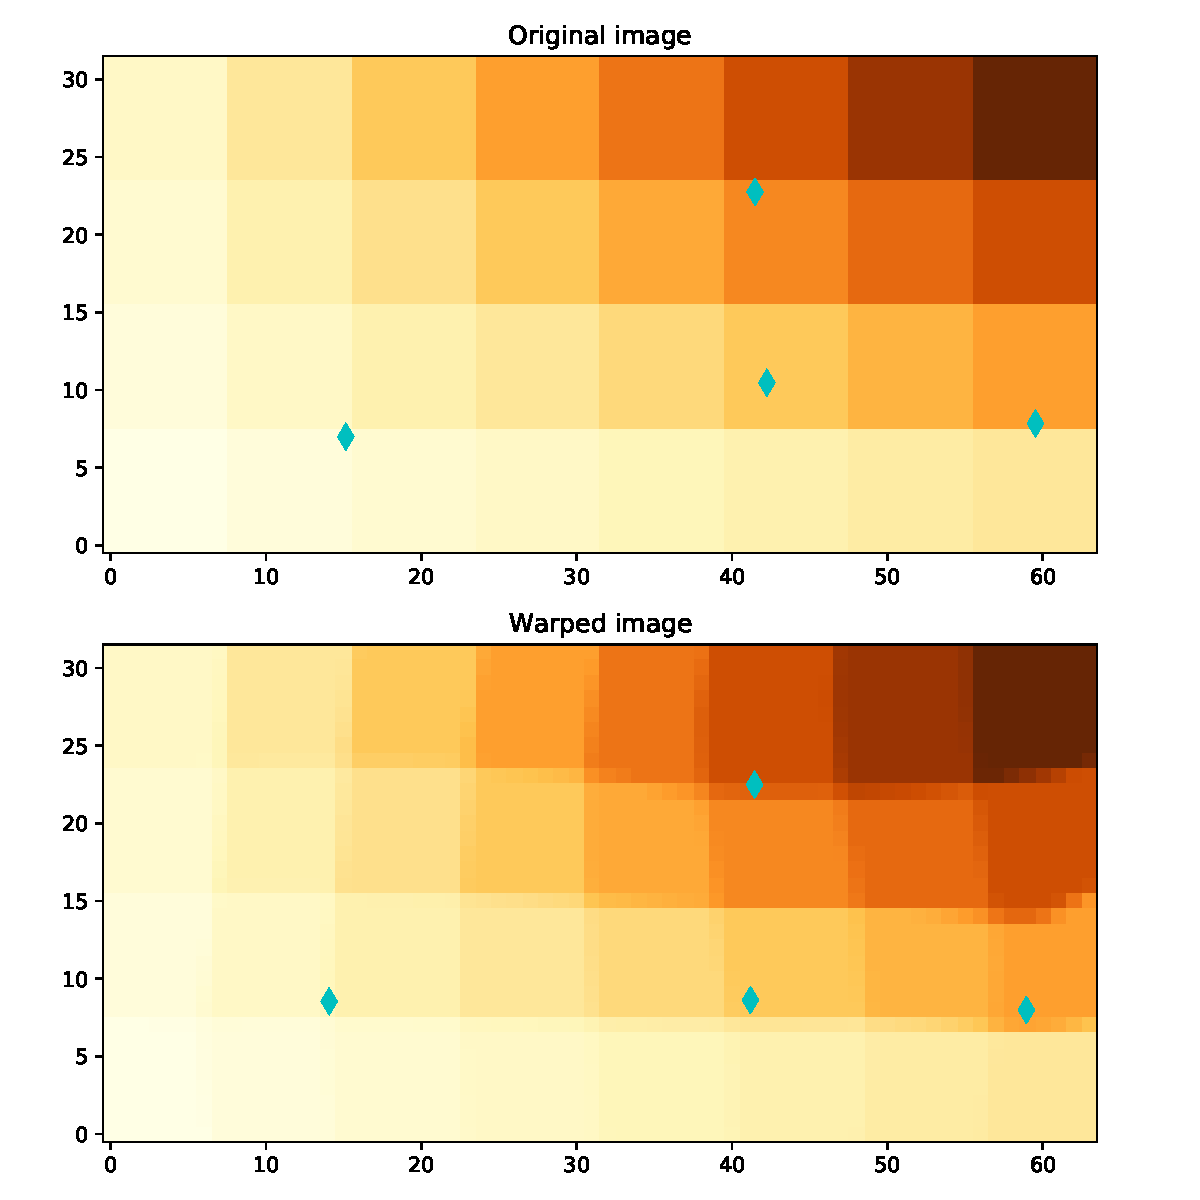
\includegraphics[width=0.9\linewidth]{warp_grid.pdf}
    \caption{
    The effects of \texttt{sparse\_image\_warp} on an image, with
\texttt{num\_landmarks} $=4$, \texttt{max\_warp\_time} $=2$ and
\texttt{max\_warp\_freq} $=2$. The diamonds show the source and destination
landmarks.}%
    \label{fig:warp_grid}
\end{figure}

\section{Learning Framework}
\label{sec:learning_framework}

The training was done using the tensorflow library \cite{tensorflow2015-whitepaper}.

Several training parameters were tweaked during the experiments to maximize the models' performance.
A brief overview of each parameter follows.

\subsection{Learning rate schedule}

\subsubsection{Finding optimal LR values}

% \begin{figure}[t!]
%     \centering
%     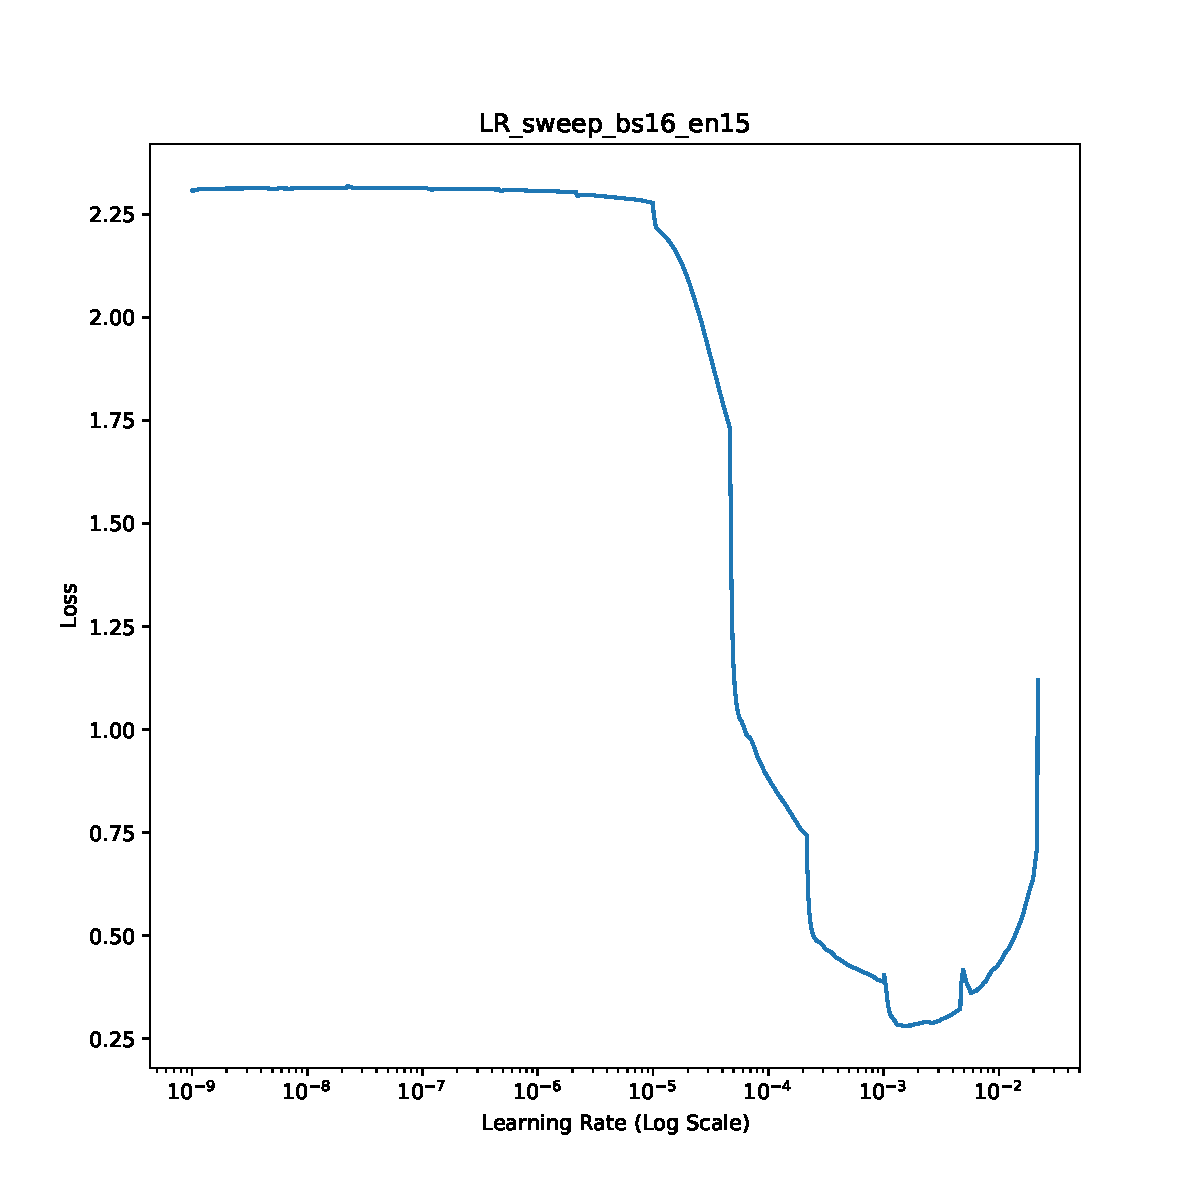
\includegraphics[width=0.9\linewidth]{LR_sweep_bs16_en15.pdf}
%     \caption{LR_sweep_bs16_en15}%
%     \label{fig:LR_sweep_bs16_en15}
% \end{figure}

% https://latexdraw.com/how-to-annotate-an-image-in-latex/
\begin{figure}[t!]
    \centering

    \begin{tikzpicture}

        % \node (image) at (0,0) {
        % \node[anchor=south west] (image) at (0,0) {
        \node[above right] (image) at (0,0) {
            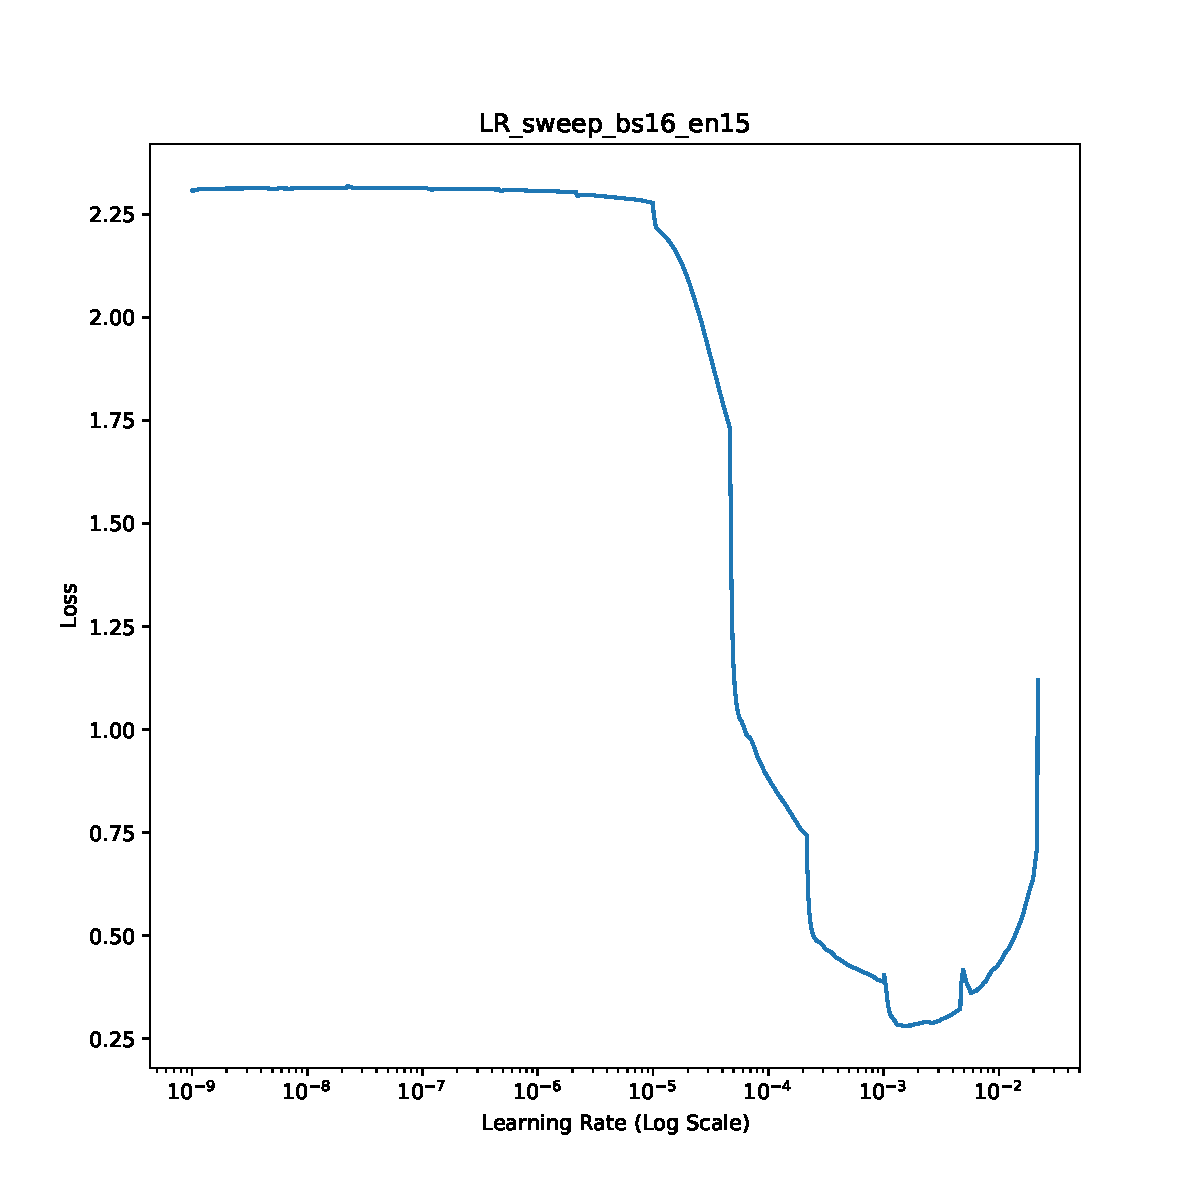
\includegraphics[width=0.9\linewidth]{LR_sweep_bs16_en15.pdf}
        };

        \draw[latex-, very thick,red] (4.3,6.4) -- ++(-1,-1.2)
            % node[left,black,fill=white]{\small Voltage source};
            % node[below left, black, fill=white, text width=2.5cm]{\small The loss starts to drop at $1e-5$};
            node[below, black, fill=white, text width=2.5cm]{\small The loss starts to drop at $1e-5$};

    \end{tikzpicture}

    \caption{LR_sweep_bs16_en15}%
    \label{fig:LR_sweep_bs16_en15}
\end{figure}


\subsubsection{Fixed LR}
\subsubsection{Exp decay LR}
\subsubsection{Cyclic LR}

\subsection{Optimizer}

\subsection{Regularization and Batch Normalization}

\subsection{Early stopping}

Loss, validation, overfitting

Show a plot

Model checkpointing

TensorBoard

\subsection{Hyper-parameter tuning}

Come lo fai

Usare Pool

Ovviamente non su tutte le combinazioni

Pay attention (no pun) to over-representation of the good params.

Epoche/batch, tempo di computazione

\section{Convolutional Neural Network}
\label{sec:convolutional_arch}

\subsection{Architecture}

As a starting benchmark, a standard Convolutional Neural Network was implemented.
Three convolutional modules are instantiated, followed by a dense classifier.
Each convolutional module is composed of the convolutional layer, a batch
normalization layer, a max pooling layer and a dropout layer.
The classifier is composed by three dense layers, the last with softmax
activation and a number of units equal to the number of classes to predict.

\subsection{Model hyper-parameters}

When building the model, aside from the number of classes to predict and the
input shape of the spectrogram, five parameters can be set:
\begin{enumerate}
    \item Number of convolutional filters: deeper layers have to learn more
        filters, as the feature maps decrease in width and height after the
        pooling.
    \item Shape of the convolutional filters:
        both square and rectangular filters were tested.
        A vertical rectangular filters (e.g. (5, 1)) emphasizes the
        relationship between mel coefficients within the same time step
    \item Shape of the pooling window: 
        both square and rectangular windows were tested.
        Again, a rectangular filter allows to push into deeper layers more
        information along the time or frequency axis.
    \item Dropout rates after the convolutional modules.
    \item Width of the dense classifier layers.
\end{enumerate}
The possible values for the hyper-parameters are:
\begin{itemize}
    \item dense\_width = [16, 32, 64, 128]
    \item filters = [10, 20, 32, 64, 128]
    \item dropout = [[0.03, 0.01],  [0.3, 0.1]]
    \item kernel\_size = [[(2,2), (2,2), (2,2)], [(5,1), (3,3), (3,3)]]
    \item pool\_size = [[(2,2), (2,2), (2,2)], [(2,1), (2,2), (2,2)]]
\end{itemize}

% hypa_grid['dataset'] = ['mfcc01' 'aug13' 'mel01' 'aug02' 'mfcc03' 'aug07' 'aug04' 'mel03'
%  'mfcc04' 'mfcc02' 'mel04' 'aug10' 'aug03' 'mel02' 'aug06' 'aug05' 'mela1'
%  'aug09' 'aug08' 'aug12' 'aug11' 'aug14' 'aug15']
% hypa_grid['words'] = ['f1' 'num' 'k1' 'w2' 'f2' 'all' 'dir']

% hypa_grid['batch_size'] = [128  32  64]
% hypa_grid['epoch_num'] = [ 60  15  16  30  59  58  61  31  62 101]
% hypa_grid['lr'] = ['default' '01' '03' '02' '06' '04' '05' 'e1']
% hypa_grid['opt'] = ['adam' 'a1' 'r1']


\section{Transfer Learning Approach}
\label{sec:transfer_learning}

\subsection{Transfer learning}

Transfer learning is a technique where a model developed and trained for a task
is modified slightly and used as a starting point for a different task.
A Convolutional Neural Network can be seen as a feature extractor composed with
a classifier.
The feature extractor is the largest part of the network, consisting in roughly
90\% of the trainable weights.
The idea behind transfer learning is to leverage the knowledge acquired
regarding the first part, extracting meaningful features from an image, and
modifying the latter, re-learning the classifier.
Training these big networks (10-100 millions of parameters) on ImageNet (14
millions of images in 1000 classes) can take from days to over a month even on
supercomputers with dozens of top of the line graphics cards.
Adapting the networks for a new task, on the other hand, is a matter of roughly
half an hour on a single GPU.

As spectrograms can be interpreted as images, starting from an image classifier
makes perfect sense. The two architecture used are Xception 
\cite{chollet2017xception}
and EfficientNet
\cite{tan2020efficientnet}.

\subsubsection{Xception structure}

A standard convolutional layer tries to learn 3D filters, with two spatial
dimensions and one channel dimension.
Such a filter has to simultaneously learn spatial correlations and
cross-channel correlations.
The Inception Hypothesis asserts that it would be easier to learn independently
the cross-channel and spatial correlations.
To do so an Inception module first learns cross-channel correlations with 1x1
convolutions, then learns spatial correlations with standard 3x3 and 5x5
convolutions.
The Xception model pushed this hypothesis to the limit, completely decoupling
the mapping of spatial and cross-channel correlations.

\subsubsection{EfficientNet structure}

Scaling a Convolutional Neural Network can lead to increased performance:
adding more layers, more filters of more convolutional modules can make the
model more accurate. On the other hand, a bigger model means slower training
and higher memory consumption to the point of being infeasible to train.
On top of that, often CNN can be over-parametrized: model compression
techniques can trade little accuracy for a great reduction in model size
\cite{han2016deep}.

The EfficientNet authors carefully examine the scaling of a model to obtain the
optimal parameters of width, depth and resolution, proposing a new compound
scaling method, which uses a single compound coefficient to scale the three
parameters in a coordinated way.
% which use a compound coefficient φ to uniformly scales network width, depth,
% and resolution in a principled way we have also developed a new mobile-size
% baseline, called EfficientNet fix φ = 1, assuming twice more resources
% available, and do a small grid search of α, β, we then fix α, β, γ as
% constants and scale up baseline network with different φ

\subsection{Transfer learning and fine tuning}

The pipeline to train a model using transfer learning is as follows:
\begin{enumerate}
    \item Load a previously trained base model, without the final classifier.
    \item Freeze the base model weights, to avoid destroying the information they
        contain.
    \item Add a classifier on top of the base model.
    \item Train the classifier, using a reasonably high learning rate.
    \item Un-freeze the base model weights.
    \item Train the model again, with a very small learning rate, to fine tune
        the feature extractor to the current dataset.
\end{enumerate}

The first four steps are the transfer learning part, followed by the fine
tuning steps five and six.

\subsection{Model building and hyper-parameters}

The inputs to the pre-trained Xception and EfficientNet models have to be
square images with three channels.
To appropriatley shape the input data, three square spectrograms were stacked
along the depth dimension.
On top of that, to obtain square inputs, two rectangular spectrograms were
concatenated horizontally (e.g. two $\left( 128, 64 \right)$ spectrogams are
composed into one $\left( 128, 128 \right)$), before being stacked.
The inputs also need to be normalized, which can be easily done with a
Normalization layer provided by tensorflow.
It is to note that the inputs should be of higher resolution (e.g. $\left( 299,
299, 3 \right)$ for Xception), whereas the spectrograms used were of size
$\left( 128, 128, 3 \right)$, so some loss of performance can be expected.
The classifier built is composed by a GlobalAveragePooling2D layer, which
averages the values in each feature extracted, followed by some dense layers
(according to the hyper-parameters selected) and finally a softmax layer to
compute the predictions.

When building the model, aside from the number of classes to predict and the
input shape of the spectrograms, two parameters can be set:
\begin{enumerate}
    \item Dropout rate after the GlobalAveragePooling2D layer.
    \item Dense width and number of the dense layers in the classifier.
\end{enumerate}
The possible values for the hyper-parameters are:
\begin{itemize}
    \item dropout\_types = [0.2, 0.1, 0]
    \item dense\_width\_types = [[4, 0], [16, 16], [0, 0], [64, 64]]
\end{itemize}
Where a value of $0$ means that the layer is skipped.

\section{Attention Model}
\label{sec:attention_model}

\subsection{Attention architecture}

The key idea behind the Attention mechanism is the assumption that not all of
the data that is available carries the same amount of information.
% Indeed, when processing a large amount of information we focus on few relevant details.
The attention mechanism allows to focus on few relevant details when presented
with large amount of data.
This approach was used effectively in the field of Neural Machine Translation
by Bahdanau \cite{bahdanau2016neural} and Luong \cite{luong2015effective}, and
to produce image captions with the Show, Attend and Tell approach
\cite{xu2016show}.

In the paper by Douglas et al. \cite{2018arXiv180808929C}, the attention
mechanism is used for speech command recognition.
The ouput shapes of each layers are reported to track along which axis the dot
multiplications are done.
As a first step, the mel spectrogram
(shape [spec\_len, nMel])
is computed from the input audio
(shape [raw\_len]).
A 2D convolution is performed, only along the time axis to extract local
correlations in the spectrogram
(shape [spec\_len, nMel, n\_filters]).
A final 2D convolution, with just one filter, condenses the information back to a 2D image
(shape [spec\_len, nMel, 1])
and the last dimension is squeezed away
(shape [spec\_len, nMel]).
Two bidirectional \cite{Schuster1997BidirectionalRN} long short-term memory
\cite{lstm} units are used to capture forward and backward long term
dependencies in the spectrogram
(shape [spec\_len, LSTM\_units*2]).
A LSTM layer reads the input sequence from the first sample to the last. The
bidirectional version reads the sequence both forward, producing the forward
hidden states, and backward, resulting in the sequence of backward hidden
states.
Now the attention mechanism is applied: one of the LSTM output vector is
selected (the choice is not crucial because the vectors should contain
information about long term dependencies) and a dense layer is used to extract
a query vector
(shape [LSTM\_units*2]).
The query vector is used to compute the attention scores, by computing the dot
product between all the LSTM outputs and the query vector along the
\textit{second} axis of the LSTM outputs, that are converted with a softmax
layer in attention weights
(shape [spec\_len]).
These weights are multiplied with the output of the LSTM along the
\textit{first} axis of the LSTM outputs to compute a weighted average of the
LSTM vectors
(shape [LSTM\_units*2]),
which is then fed into a dense classifier
(shape [nClasses]).
In this way, the output vector of the LSTM is not just the final hidden state,
but it is a function of all the hidden states, where the most important states
are given more relevance, according to the attention weights.

\subsection{Query style}

Two additional methods to compute the query were developed and tested.
In the first method, from the output of the second LSTM layer, a CNN was used
to extract the query, using several convolutional modules.
In the second method, the query was directly computed from the input
spectrogram, using a CNN.
A third query style tested is regarding the choice of LSTM output vector to
pick to compute the query: instead of the last, the central vector was chosen.

TODO: un grafichetto sarebbe bellissimo

\subsection{AreaNet}

Dream a dream

\subsection{Model building and hyper-parameters}

When building the model, aside from the number of classes to predict and the
input shape of the spectrograms, six parameters can be set:
\begin{enumerate}
    \item Number of convolutional filters in the convolutional modules.
    \item Dropout rate after the convolutional modules.
    \item Shape of the convolutional filters:
        both square and rectangular filters were tested.
        A vertical rectangular filters (e.g. (5, 1)) emphasizes the
        relationship between mel coefficients within the same time step
    \item Number of LSTM units.
    \item Query style: either a single output vector from the LSTM or the
        result of a convolutional operation, that takes as input the original
        spectrogam or the vectors produced by the LSTM.
    \item Width of the dense classifier layers.
\end{enumerate}
The possible values for the hyper-parameters are:
\begin{itemize}
    \item conv\_size = [[10, 0, 1], [10, 10, 1]]
    \item dropout = {0.2, 0}
    \item kernel\_size = [[(5,1), (5,1), (5,1)], [(3,3), (3,3), (3,3)]]
    \item lstm\_units = [[64, 64], [64, 0]]
    \item query\_style = ["dense01", "dense02", "conv01", "conv02", "conv03"]
    % \item query\_style = [\texttt{dense01}, \texttt{dense02},
    % \texttt{conv01}, \texttt{conv02}, \texttt{conv03}]
    \item dense\_width = [32, 64]
\end{itemize}

